
\subsection{New Methodology Overview \todo{Adopt from Section 5.2.2}}
\label{sec:intro-adapt-method}
% There are mainly three challenges in order to analyze this adaptivity property, 
% and the full-spectrum 
The analysis framework for the adaptivity property is 
% In this proposal, I will first focus on analyzing 
% this adaptivity property for the program based on solving 
developed w.r.t. the three challenges introduced above accordingly.
As shown in Figure~\ref{fig:structure}.
% There are mainly three parts, each targeting on a challenge above.
It is composed of three parts, with each targeting on a challenge above.
The fundamental part is the {\tt Query While} language designed for formalizing the 
adaptive data analysis. Built on this, 
the execution-based adaptivity analysis (targeting to the \emph{adaptivity} formalization challenge)
and the static program analysis (targeting to the \emph{adaptivity} estimation challenge) 
are the two analysis parts of this 
% full-spectrum 
% adaptivity 
analysis framework.
\begin{figure}
   \centering   
   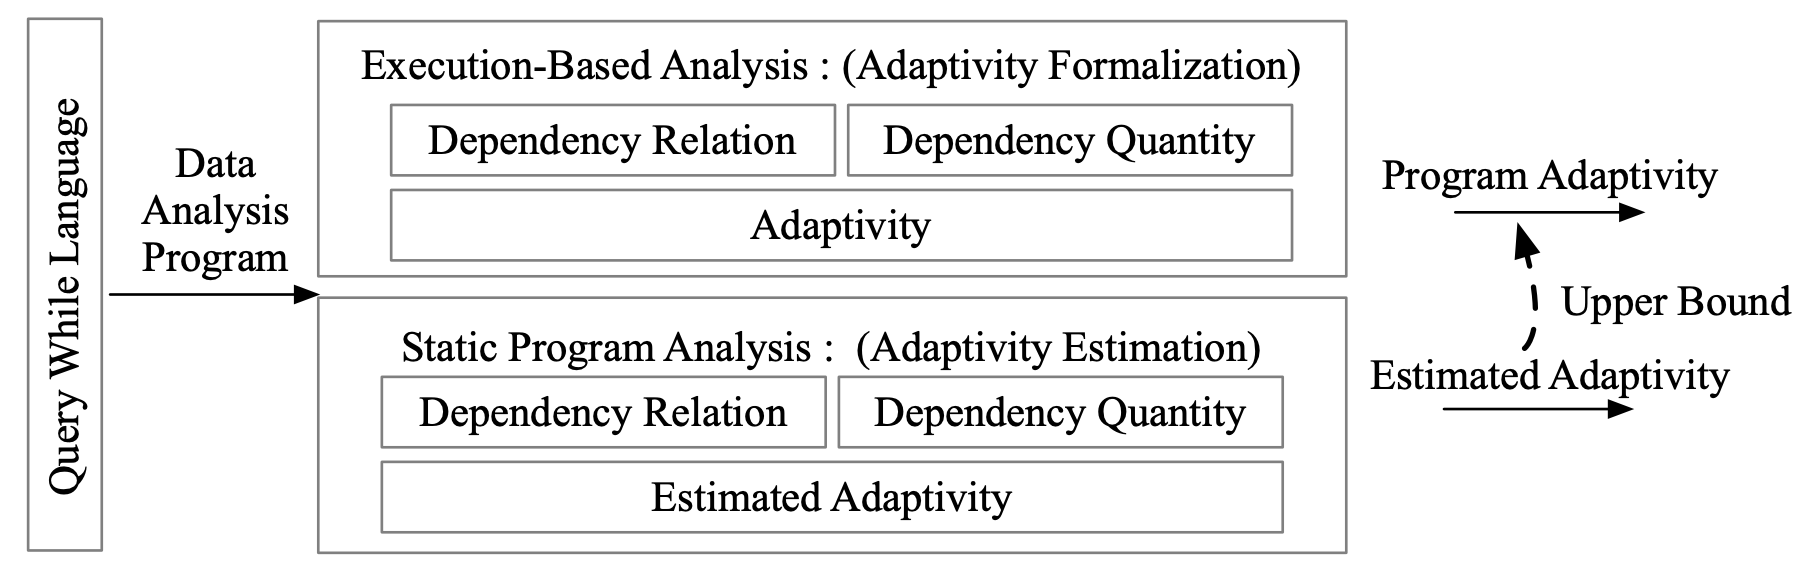
\includegraphics[width=1.0\textwidth]{figures/overview.png}
  \caption{High level architecture of the Program Analysis Framework}
   \label{fig:structure}
\end{figure}

\begin{enumerate}
 \item
 \textbf{Adaptive Data Analysis Formalization}
% The first challenge is \emph{how to define formally} a model for adaptive data analysis which is general enough to support the methods I discussed above and would permit to formulate the notion of adaptivity these methods use. 
% I take the approach of designing a programming framework for submitting queries to some \emph{mechanism} giving access to the data mediated by one of the techniques I mentioned before, e.g., adding Gaussian noise, randomly selecting a subset of the data, using the reusable holdout technique, etc. 
% In this approach, a program models an \emph{analyst} asking a sequence of queries to the mechanism. The mechanism runs the queries on the data applying one of the methods discussed above and returns the result to the program. The program can then use this result to decide which query to run next. 
% % Overall, I am interested in controlling the generalization of the results of the queries which are returned by the mechanism, by means of adaptivity. 

% \textbf{Methodology}
% Motivated by this,
In order to define formally a model for adaptive data analysis,
I present a while-like language named {\tt Query While}
with extensions on query requests in Section~\ref{sec:language}.

\item 
\textbf{Adaptivity Formalization}
% The second challenge is \emph{how to define the adaptivity of a given program}.
% Intuitively, a query $Q$ may depend on another query $P$, if there are two values that $P$ can return which affect in different ways the execution of $Q$. 
% For example, as shown in \cite{dwork2015reusable}, and as I did in our example in Figure~\ref{fig:generalization_errors}(a), one can design a machine learning algorithm for constructing a classifier that first computes each feature's correlations with the label via a sequence of queries, and then constructs the classifier based on the correlation values. 
% If one feature's correlation changes, the classifier depending on features is also affected. 
% This notion of dependency builds on the execution trace as a \emph{causal history}. 
% In particular, I am interested in the history or provenance of a query up until this is executed, I am not then concerned about how the result is used --- except for tracking whether the result of the query may further cause some other query. 
% This is because I focus on the generalization error of queries and not their post-processing. % 

% \textbf{Methodology}
% To formalize 
In order to give a formal model for this intuitive \emph{adaptivity} as a quantitative program property, 
I develop an execution-based analysis in Section~\ref{sec:dynamic}.
% I first consider all the possible evaluations of a program --- I do this by 
% I use a trace semantics recording the execution history of programs on some given input --- and I create a dependency graph, where the dependency between different variables (query is also assigned to a variable) is explicit and track which variable is associated with a query request. 
% I then enrich this graph with weights describing the maximal number of times each variable is evaluated in a program evaluation starting with an initial state. The adaptivity is then defined as the length of the walk visiting most query-related variables on this graph. 
% Through two aspects: the execution-based analysis and static-based program analysis.
% In the execution-based analysis, I will formalize the intuitive notion of \emph{adaptivity} as a quantitative 
% property of programs. This analysis is developed 
 This execution-based analysis is designed in three steps through different methodologies as follows,
 \begin{enumerate}
 \item The first step is to analyze the \emph{dependency relation} between every query, 
 through the methodology of semantic data dependency analysis.
 %
 Specifically through a trace semantics recording the execution history of programs on given input,
 % --- and I create a dependency graph, 
 the dependency between different variables (query is also assigned to a variable) is explicitly tracked and 
 analyzed.
%   and 
%   which variable is associated with a query request. 
% I then enrich this graph with weights describing the maximal number of times each variable is evaluated in a program evaluation starting with an initial state. The adaptivity is then defined as the length of the walk visiting most query-related variables on this graph. 
% In the execution-based analysis, I will formalize the intuitive notion of \emph{adaptivity} as a quantitative 
% property of programs. This analysis is developed 
% \\
 \item The second step is to analyze the \emph{dependency quantity} 
%  analysis, 
based on the \emph{dependency relation} above.
This analysis is developed through the methodology of execution-based reachability bound analysis.
% \\
 \item The last step is the intuitive \emph{adaptivity} quantity analysis, 
 according to the two analysis results above, specifically \emph{dependency relation} and \emph{dependency quantity}.
 This step 
%  is developed through 
gives the formal \emph{adaptivity} definition as the analysis result. \\
 Specifically, this analysis is developed through creating a dependency graph firstly. 
 In this graph, the dependency between different variables (query is also assigned to a variable) 
 is explicit and track which variable is associated with a query request. 
 This dependency comes from the \emph{dependency relation} from the first step analysis.
 \\
Then, I enrich this graph with 
weights describing the maximal number of times each variable is evaluated 
% in 
% a program evaluation starting 
during the program execution, w.r.t. an initial state. 
This weight comes from the \emph{dependency quantity} from the second step analysis results.
\\
 The adaptivity is then defined as the length of the walk visiting most query-related variables on this graph. 
 \end{enumerate}
\item 
\textbf{Adaptivity Estimation}

% The third challenge is \emph{how to estimate the adaptivity of a given program}. 
% The adaptive data analysis model I consider and our definition of adaptivity suggest that for this task I can use a program analysis that is based on some form of dependency analysis. This analysis needs to take into consideration:
% 1) the fact that, in general, a query $Q$ is not a monolithic block but rather it may depend, through the use of variables and values, on other parts of the program. 
% Hence, it needs to consider some form of data flow analysis. 
% 2) the fact that, in general, the decision on whether to run a query or not may depend on some other value. Hence, 
%  it needs to consider some form of control flow analysis.
% 3) the fact that. in general, I am not only interested in whether there is a dependency or not, but in the length of the chain of dependencies. 
% Hence, it needs to consider some quantitative information about the program dependencies. 
% {A quick example is that: I store the result of query $Q_1$ in variable $x$ and use variable $y$ to record the result of query $Q_2$. I want to construct the third query $Q_3$ which relies on the value stored in $x$, let us say, $Q_3$ will ask for the sum of the first column of a table if $x$ is positive and the sum of the second column otherwise. In this situation, I need data flow analysis. On the other hand, if I need the value of $y$ to help us decide whether I should ask $Q_3$, for example, I ask the third query if $y$ is odd, and do not ask if $y$ is even. Naturally, to be able to handle this case, control flow analysis comes into play. Formally speaking, }
% \textbf{Methodology}
% To address 
In order to give an accurate estimation on the adaptivity of a given program, and address
the challenges of the \textbf{Adaptivity Estimation},
% considerations and be able to estimate a sound upper bound on the adaptivity of a program, 
I will develop a static program analysis in Section~\ref{sec:static}, named {\THESYSTEM}.
This analysis combines data flow and control flow analysis with reachability bound analysis.
% ~\cite{GulwaniZ10}. 
This new program analysis gives tighter bounds on the adaptivity of a program than the ones one would achieve 
by directly using the data and control flow analyses or the ones that one would achieve 
by directly using reachability bound analysis techniques alone. 
% Specifically as follows in the same 
It is developed in 3 aspects similar to the execution-based analysis 
while through static program analysis techniques.
A sound estimated result is given in each part, which is summarized as follows.
\begin{enumerate}
\item The data dependency relation analysis through the static data flow analysis technique.
\item The dependency quantity analysis through the static program reachability bound analysis techniques.
\item 
% The program  estimation, 
The static analysis for adaptivity, specifically estimating the \emph{adaptivity} formalized in the execution-based analysis.
%  is presented in Section~\ref{subsubsec:static-reachability}.
% the program adaptivity estimation, 
In this analysis, I construct a program-based dependence graph for approximating the execution-based graph
%  in Section~\ref{subsubsec:dynamic-adapt}.
Then, based on this graph, I design an algorithm
%  based on the results estimated above, 
computing the adaptivity upper bound soundly 
and accurately.
\end{enumerate}
%%%%% To reason about%
\end{enumerate}% \\


Based on the implementation and experimental results of the program analysis framework,
%  on the $\THESYSTEM$,
I plan to focus on the following three further features which can be extended and improved.
%  in my full-spectrum analysis.
\begin{enumerate}
    \item In the adaptive data analysis formalization, I plan to extend the {\tt Query While} Language with inter-procedure call.
    \item In the execution-based \emph{adaptivity},
    I plan to improve the precision of the \emph{adaptivity} formalization w.r.t. the program's intuitive adaptivity rounds,
%  in the formal  model 
and extend this analysis with inter-procedure call.
\item In static \emph{adaptivity} analysis, I plan to give a tighter estimated upper bound on \emph{adaptivity}.
%  give a tighter estimated upper bound 
Specifically, I will focus on improving the accuracy of the static \emph{dependency quantity} analysis in the second step through 
developing a new path sensitive reachability bound analysis technique. 
% \item In the third step of static program analysis, I will improve the accuracy of the adaptivity computation algorithm,
% compute a tighter adaptivity upper bound as well.
\end{enumerate}